\documentclass[a4paper,12pt]{article}%
\usepackage[utf8]{inputenc}%
\usepackage[margin=0.7in]{geometry}%
\usepackage[spanish]{babel}%
\usepackage{graphicx}%
%
\title{REPORTE AUTOMÁTICO DE ACTIVIDAD VOLCÁNICA EN ALTO BIO{-}BIO}%
\title{REPORTE AUTOMÁTICO DE ACTIVIDAD VOLCÁNICA EN ALTO BIO{-}BIO}%
\author{ENEL {-} Universidad de Concepción}%
\date{01 de April de 2019 (21:26:56 UTC)}%
%
\begin{document}%
\pagestyle{empty}%
\normalsize%
\maketitle%
La CENTRAL DE MONITOREO DE ACTIVIDAD VOLCÁNICA da a conocer la siguiente información obtenida a través de los equipos de monitoreo en tiempo real de ENEL {-} UNIVERSIDAD DE CONCEPCIÓN:\newline%
\newline%
%
Hoy 25 de March de 2019 a las 00:00:00 hora UTC (hora local = UTC {-} 03:00), las estaciones sismológicas instaladas en Alto Bio{-}Bio detectaron automáticamente un evento sísmico de magnitud local 0.0, el cual está localizado a 0.0 km de profundidad. Los datos de localización son los siguientes: \newline%
\newline%
%


\begin{figure}[ht!]%
\centering%
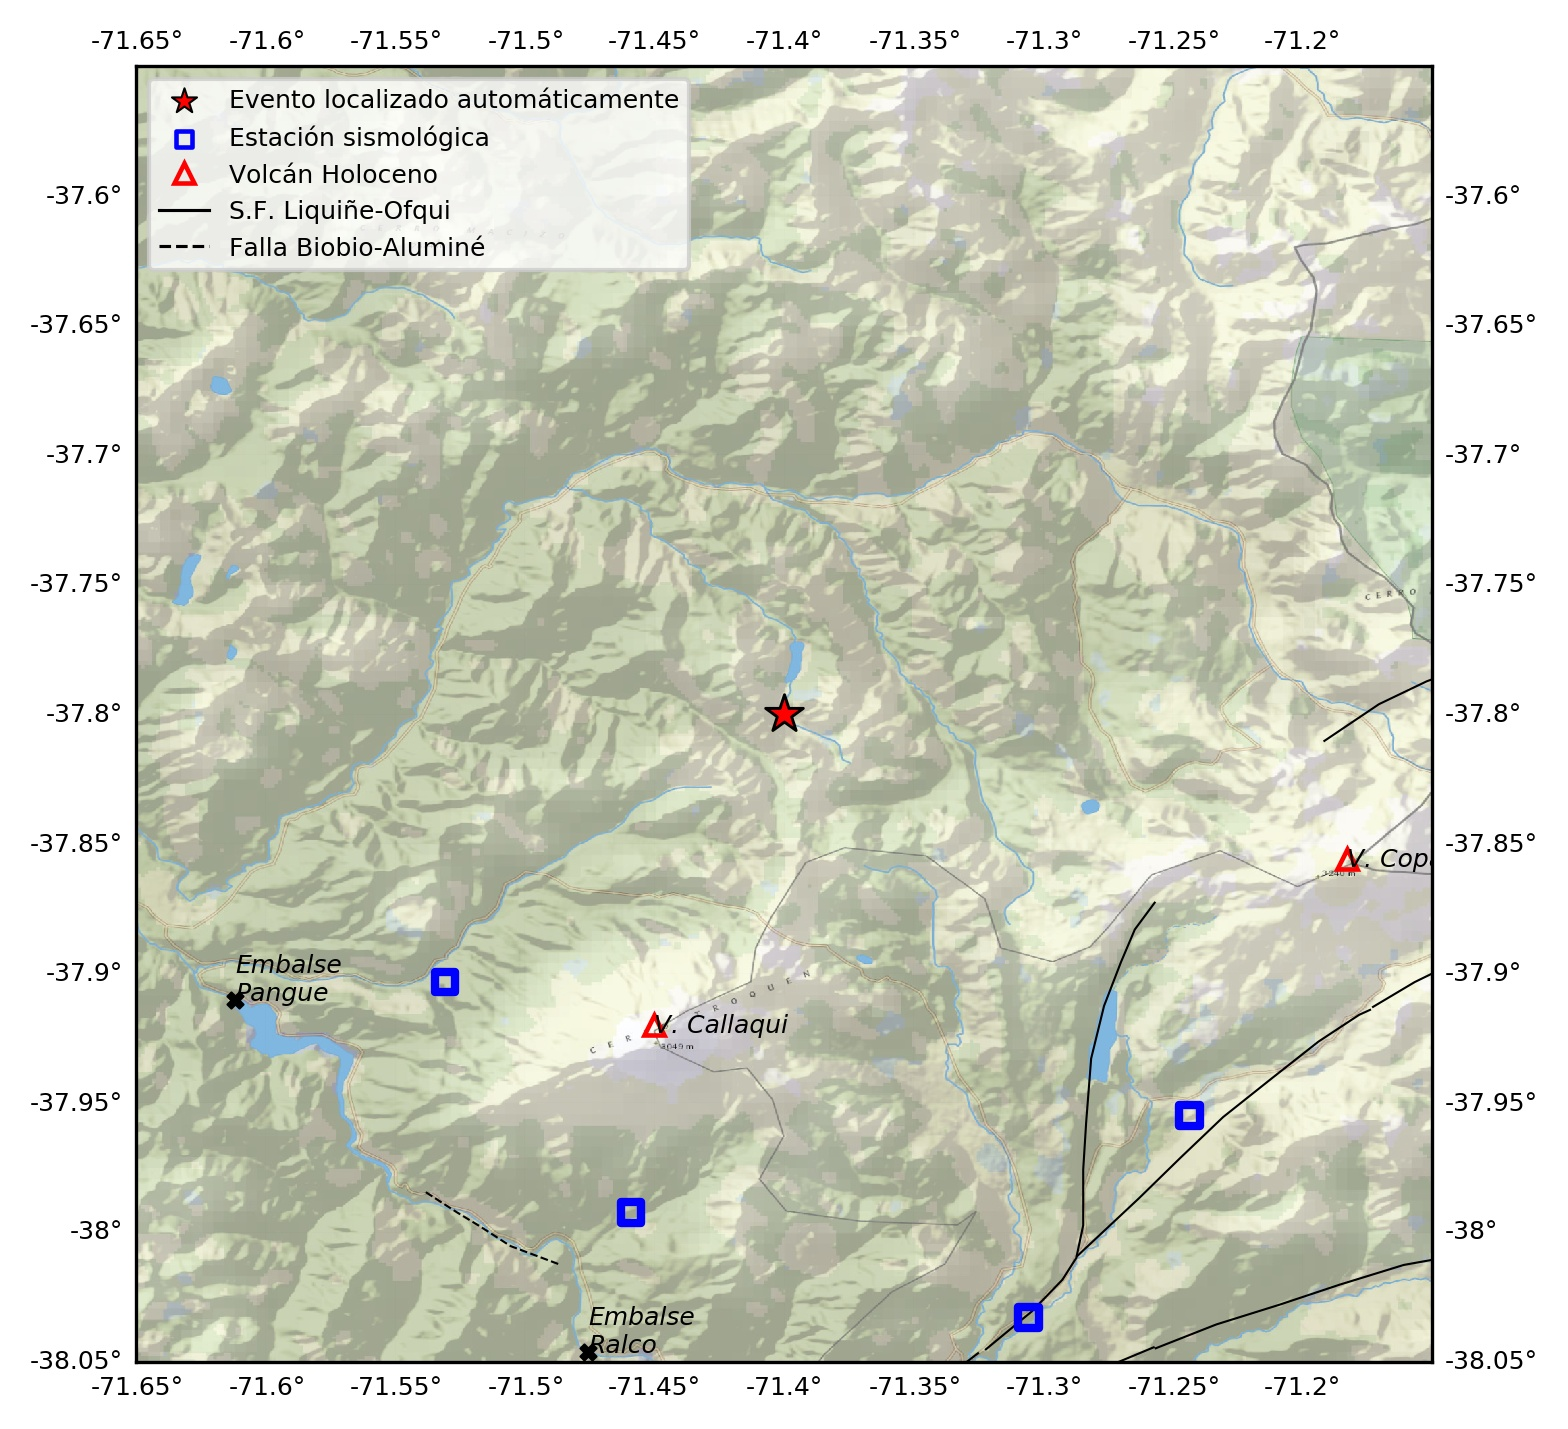
\includegraphics[width=0.8\textwidth]{figs/map_automatic.jpg}%
\end{figure}

%


\begin{figure}[ht!]%
\centering%
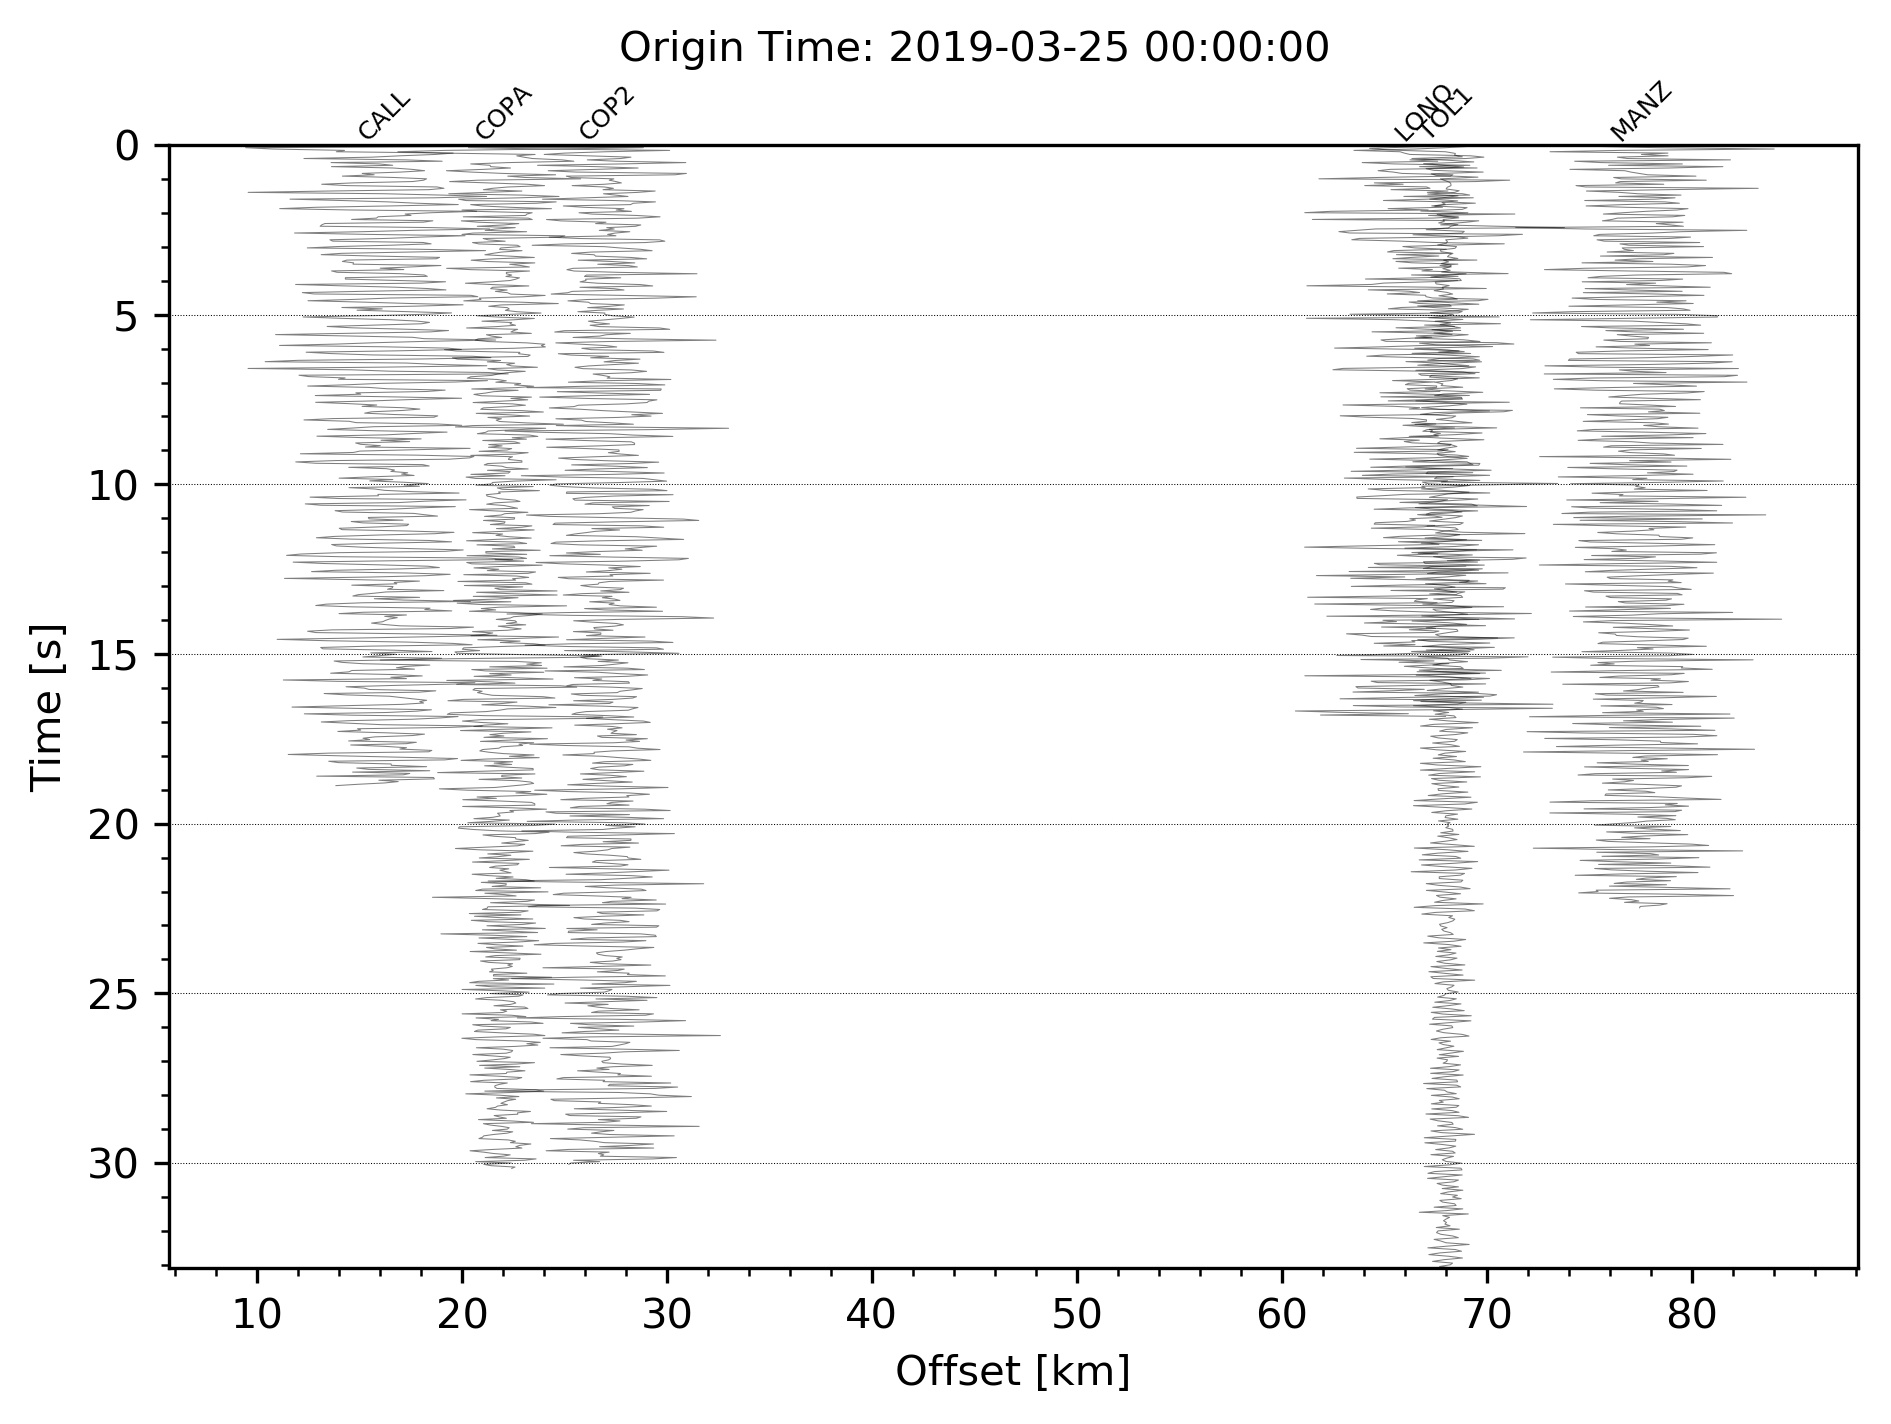
\includegraphics[width=0.7\textwidth]{figs/waveforms_automatic.jpg}%
\end{figure}

%
\newline%
\newline%
\newline%
TIEMPO DE ORIGEN: 2019{-}03{-}25 00:00:00 UTC\newline%
MAGNITUD: 0.0\newline%
LONGITUD: {-}71.4000\newline%
LATITUD: {-}37.8000\newline%
PROFUNDIDAD: 0.0 km\newline%
ESTACIONES: 0\newline%
GAP: 0.0\newline%
RMS: 0.0\newline%
%
IMPORTANTE: Los datos mostrados en este reporte son generados automáticamente y deben ser revisados por un analista. Cualquier consulta dirigirla directamente a:\newline%
%
Email: gemaudec.concepcion@gmail.com%
\end{document}